%Chapter 4: Kinematic Source Inversions

\chapter{Kinematic Source Inversions}

In Chapter 3 we discussed a framework for static slip inversions. Elaborating on the work of \citet{Crowell2012} we demonstrated it is possible to construct static models for large earthquakes objectively with minimal interaction from a human operator. Static dislocation models are limited in the sense that they provide only the total slip on the assumed rupture surface and provide no information on the time evolution of rupture. They are just a before and after snapshot of the event.  They do not illuminate important kinematic parameters of the rupture process; how fast was the rupture? What is the shape of the source time function, both at individual sub-faults and for the earthquake as a whole? Answers to questions like these have important implications not only for hazards applications but to furthering our understanding of the physics that governs the rupture process.

\section{Background}

\label{sec_backgr}

As instrumental seismology matured in the mid 20th century and observatory grade seismological stations and strong motion sensors proliferated it became possible to consider kinematic models of the earthquake source process. Perhaps the first successful macroscopic model, containing simple parameters, was the Haskell fault model \citep{haskell1964,haskell1969} which consisted of a rectangular fault with constant, unidirectional rupture velocity (a boxcar source time function). It successfully explained phenomena such as directivity and made predictions about the shape of source spectra. This propagating dislocation model was successfully used to model data observed at only 80m from the fault trace of the 1966 Parkfield earthquake \citep{aki1968}.

As systematic studies of source properties evolved it became apparent that large earthquakes had more complexity than a simple propagating line source with a prescribed rise time and rupture velocity and homogenous slip. Indeed it was clear that some events could only be modeled by relaxing these constraints. \citet{kanamori1978} demonstrated that the far field body waves of the 1976 $M_w$7.6 Guatemala earthquake were best explained by superposition of ten sources, while \citet{trifunac1974} employed strong motion records of the 1971 $M_w$ 6.6 San Fernando earthquake to solve the first heterogeneous slip inversion proper.

Following the 1979 $M_w$6.4 Imperial Valley earthquake, which was well recorded by numerous strong motion stations, an efficient way to parametrize the temporal and spatial variations of the source and invert for them was defined. \citet{olson1982} and \citet{hartzell1983} introduced what is now known as the \textit{multi-time window} method, whereby slip on a sub-fault is allowed to occur over contiguous time windows. In this way heterogeneities of the spatial and temporal behavior of the fault can be modeled.

Formally, an inversion problem for the time dependent slip of an earthquake can be set-up by discretizing an assumed fault surface into a grid of $N$ sub-faults. Then, the response at a given station can be computed from
\begin{equation}
\label{eq:slip}
u(t)=\sum_{j=1}^ND_j[\cos(\lambda_j)G_j^{ss}(v_j,t)+\sin(\lambda_j)G_j^{ds}(v_j,t)]\dot{S}_j(t)\;,
\end{equation}
where $u(t)$ is the displacement seismogram at a given station and $D_j$ the dislocation amplitude at the $j$-th sub-fault. The dislocation is decomposed into its strike-slip ($ss$) and dip-slip ($ds$) contributions by taking the cosine and sine, respectively, of the rake angle $\lambda$. $G^{ss}(v,t)$ and $G^{ds}(v,t)$ are the dip-slip and strike-slip Green functions which represent the response of a point, impulsive source. $\dot{S}(t)$ is the source time function which regulates the temporal dependence of moment release at a subfault. The Green functions depend on the rupture velocity, $v$ insofar as they need to be delayed by the time required for the rupture to propagate from the hypocenter to each subfault. Evidently, if the timing of slip is considered an unknown quantity, then the general expression in Equation \ref{eq:slip} is non-linear. Furthermore the source time function itself must be parametrized, the choice of such parametrization will also have an effect on the linearity of the problem.

Indeed, the main difference in the approaches to the kinematic slip inversion is that of the assumption of linearity. To treat Equation \ref{eq:slip} as linear one can assume a rupture speed  and allow slip at each sub-fault to happen in one or many subsequent time windows following the main arrival of the rupture front \citep{olson1982,hartzell1983}. The source time function can be parametrized in a number of ways, usually overlapping triangles or boxcars, but is in general treated as being decomposed into basis functions \citep{ide1996}. In this way the inversion is linear an can be solved with any of the usual algorithms. Typically a nonnegative least squares (NNLS) solver is employed \citep{lawson1974} to prevent the direction of slip from reversing. In this inversion approach it is important to have sufficient time windows, or basis functions, to allow for some complexity in the time evolution of slip. If the parametrization is overly simple then unexpected errors can occur in the final result \citep{hartzell1993}.

If the timing of slip is treated as an unknown quantity the non-linear inverse problem can be solved provided one assumes a parametrization of the source time function $\dot{S}$. Thus, in this approach the rupture is linear with regards to the amount of slip but non-linear with regards to its timing. Of benefit in this inversion scheme is that source time functions whose shape is based on rupture dynamics can be used. Examples of this can be found in \citet{beroza1988} who use a source time function derived from dynamic crack propagation and \citet{ji2003} who use a source time function that simulates a starting and stopping phase. Non-negativity can still be enforced in the non-linear case by employing an error function that grows asymptotically as slip approaches 0 \citep{yoshida1990}. These non-linear approaches however, use only one time window per subfault and cannot model complex source time histories. The importance of this remains unclear, there is uncertainty as to the robustness of complex source time functions obtained with the linear method. \citet{ide2007} compared several linear and nonlinear inversions for the $M_w7.6$ Chi-Chi, Taiwan earthquake and found that while the gross features of slip are consistent amongst studies there can be significant variations in the timing of slip. \citet{ide2007} also found that models that include geodetic data show improved consistency.

There is also a class of slip inversions that analyzes the data in the frequency domain. This has been a less popular but well studied approach. The first solutions in the frequency domain were reported by \citet{olson1988} and \citet{cotton1995}. Later \citet{ji2002} proposed a more innovative approach by using wavelet analysis to quantify the contributions of finite frequency signals to the slip inversion. These methods, as well as the time domain ones, independently of the data type used, far- or near-field, rely on low pass filtered time series, they depend on the long period component of the seismic record for the inversion. This choice of data type can have an effect on the final model, furthermore, whether the time series are studied as velocity or displacement waveforms can also affect the inversion result \citep{ide2007}. velocity waveforms tend to display higher levels of high frequency waves, while displacement waveforms are dominated by long period energy. Due to this large suite of options available to the seismologist who wishes to study the time dependent behavior of earthquake rupture, there is still a lot of heterogeneity in the results reported by independent research groups for any given earthquake. Nonetheless, kinematic inversion has become a routine analysis and important tool for the study of medium to large events.

For rapid response the USGS routinely produces automated slip inversions for large events using the wavelet method of \citet{ji2002} and relying on far field body and surface waves. These models are computed several hours after the event and are usually the first source of kinematic information about large events. Inversions with regional data are only performed in post processing. They typically rely on baseline corrected or high-pass filtered strong motion data. Recently, for example, \citet{suzuki2011} inverted strong motion data from the $M_w$9 Tohoku-oki event using the multi-time window method. In that study the acceleration waveforms were integrated once to velocity and band-pass filtered between 100s and 8s. The results show a smooth slip distribution with large slip near the trench. However, approaches such as this one for regional inversions are limited. Consider figure \ref{fig_myg011} where we have applied a bandpass filter between 100s and 8s to the east component of station MYG011. This is the same procedure as that in \citet{suzuki2011} (station MYG011 was used in that inversion). The figure shows the filtered accelerogram integrated to velocity and then displacement. Notice that the filtering operation has eliminated the static field and the integrated displacement waveform compares very poorly to the collocated GPS station. it is not mentioned in that study how the smoothing parameters were selected, but, it is difficult to consider a model which does not constrain the static field a robust one. it is still informative, but, for certain applications, such as tsunami modeling not of much use.

An alternative approach is to directly invert high-rate GPS data. Given the problems with signal aliasing discussed in Chapter 2 and the elevated noise levels, especially in the vertical channel it is only advisable to invert the longer period portion of the GPS recording. For example \citet{yue2011} low-pass filtered GPS recordings of the Tohoku-oki event at 80mHz. This approach yields very smooth models which tend to be very similar to simple static models derived just from coseismic offsets. It is easy to understand why; at such long periods the largest signal in the time series is the coseismic ramp. Higher frequency waves are obscured and there is only limited information about the time dependent rupture process. Differentiating the GPS time series to velocity is not advisable because of the slow sampling rates and high noise.

Thus the Kalman filter solution which provides both reliable velocity and displacement waveforms that contain information across a broad frequency range seem well suited for kinematic inversion at regional distances. We will demonstrate in the following pages that this is indeed the case.

\begin{figure}[!ht] 
  \centering
  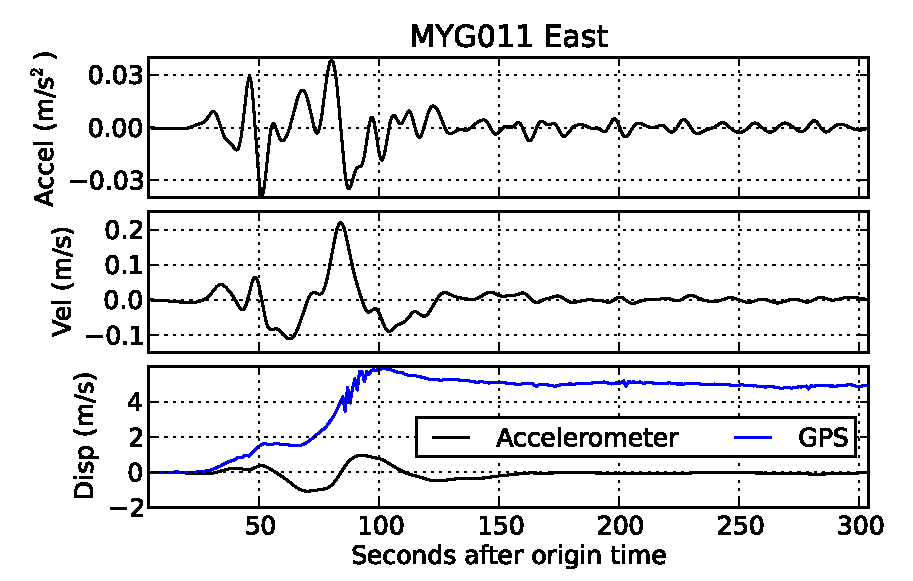
\includegraphics[width=0.8\linewidth]{./figures/ch4/myg011_vel.pdf}
    \caption[Bandpass filtered waveforms for MYG011]{Results of bandpass filtering the accelerometer recording at station MYG011 and integrating it to velocity and displacement}
  \label{fig_myg011}
\end{figure}


\section{The Inverse Problem}

Throughout this chapter we will employ for our analysis the multi-time window method. Following \cite{ide1996} we can consider the decomposition of the source time function at the $j$-th subfault into $K$ basis functions
\begin{equation}
D_j\dot{S}_j(t)=\sum_{k=1}^Kb_k\phi_k(t)\;,
\end{equation}
where $b_k$ is the expansion coefficient of the $k$-th basis function $\phi_k(t)$. In the multi-time window approach we consider overlapping basis functions with a simple geometry. Commonly used are b-splines with equally spaced knots which yield a simple isosceles triangle shape \citep{ide1996,wu2001}. 
Thus, one assumes a maximum rupture velocity $v^{max}$ and then allows slip on subsequent \textit{windows}  which are offset at regular time intervals, typically 50\% of the of the rise time of the triangle basis function. In this way we've effectively linearized the problem by assuming known rupture times, while still allowing flexibility in the timing of slip by permitting dislocations at later times after the maximum rupture velocity time. The inverse problem will now be a solution for the expansion coefficients $b_k$ which represent the amplitude of each triangle source time function at each sub-fault for strike- and dip-slip motions yielding a total of $2KN$ model parameters.


Green's functions must be computed numerically. If one assumes Earth structure is a 1D layer-cake model then at regional distances (hundreds to a couple thousand kilometers) GFs can be obtained by the frequency-wavenumber (fk) integration method \citep{saikia1994}. Importantly, the fk method is capable of computing the ultra-long period band of the seismogram down to the 0 frequency static offset \citep{zhu2002}. It can be employed to model strong motion displacement data from the seismogeodetic solution. Other approaches involve normal mode summation \citep{yue2011}. Ideally it would be desirable to use three dimensional GFs for the inverse problem solution. This is a computationally intensive operation, sometimes prohibitively so. However, it is becoming prevalent to use fully 3D Earth models for forward computation of wave propagation \citep{bielak2010,tromp2010}. As our knowledge of Earth structure progresses it will become important to consider more complex velocity models. However, 3D velocity models only exists for a very small fraction of the Earth and while \citet{graves2001} and \citet{wald2001} demonstrated that 3D structure enhances model resolution, they also showed that this improvement is only possible with accurate 3D models. In fact they demonstrated that a well calibrated 1D model is preferable over an imprecise 3D Earth model.

Thus, with Green functions in hand we can set up the traditional linear inverse problem, as in Chapter 3:
\begin{equation}
\label{eq:inv}
\mathbf{GM}=\mathbf{d}\;,
\end{equation}
where the data column-vector $\mathbf{d}$ is the concatenation of observed seismograms at all stations, the Green functions $\mathbf{G}$ are the motions at every station from every subfault for a triangle source time function of given rise-time and the model parameters $\mathbf{m}$ are the amplitude of the allowed source time functions at each sub-fault. As in the static case $\mathbf{G}$ is not full rank. Even though this is an over-determined problem the data are not always independent and parts of the model often cannot be resolved by the data. This rank deficiency produces a large condition number which effectively yields extremely irregular models with sharp, unphysical variations between neighboring subfaults and overlapping time windows. Regularization must be employed; one popular form of regularization in slip inversions is to fix the total amount of seismic moment at a value suggested from other sources \citep{ji2002b}. However for our case we prefer moment be determined by the data themselves. Rather, we employ a spatial and a temporal regularization to increase the effective rank of the problem. For the spatial regularization we use the Laplacian finite difference operator as in the static case of Chapter 3. We request that the sum of the slip of all windows at a given sub-fault be smooth in this sense. This penalty function is applied only to the total slip, not to the individual time windows. For a temporal regularization we apply a simple first derivative penalty function to each subfault's windows, such that sharp variations between the amplitudes of contiguous time-windows are possible but discouraged. 

\subsection{Spatial Regularization}

\label{sec:regu}

For slip inversions we have relied on the finite difference Laplacian operator for spatial regularization. For static inversions in Chapter 3 we used the traditional 5 point stencil approximation to the Laplacian. At a given sub-fault (position $i,j$) the 4 neighboring sub-faults are used to compute the finite difference Laplacian of a given component of  slip $m_{ij}$ as
\begin{equation}
\label{eq_laplace1}
\nabla^2m_{i,j}=\frac{-4m_{i,j}+m_{i+1,j}+m_{i-1,j}+m_{i,j+1}+m_{i,j-1}}{h}\;,
\end{equation}
where $h$ is the distance between the centers of the sub-faults. If it is constant then the term can be treated as unity. This formulation is easily derived by applying the second order accurate expressions for the second derivative in the along strike and along dip directions.  The situation is illustrated schematically in Figure \ref{fig_stencil} and the computational molecule for a slip patch within the model is in Figure \ref{fig_molecules}a  A survey of the literature will reveal that seldom do authors indicate what course of action to take at the edges of the model. At the boundaries of the fault one can simply drop one term of Equation \ref{eq_laplace1} (or two if you are at a corner). For example at the top edge of the fault model  (Figure \ref{fig_stencil}, position $i,1$) we would write
\begin{equation}
\label{eq_laplace2}
\nabla^2m_{i,1}=\-4m_{i,1}+m_{i+1,1}+m_{i-1,1}+m_{i,2}+0\;,
\end{equation}
where we have set $m_{i,0}=0$. This simplifies the computational molecule from 5 elements to 4 (Figure \ref{fig_molecules}b). Indeed, this is equivalent to assuming that there exists a ghost cell $m_{i,0}$ beyond the edge of the fault model that has no slip. This is a reasonable assumption for a buried fault where slip must taper off towards the edges. This regularization, while not precluding slip at the fault boundary, will put a large penalty on it. Large slip at the edge will mean a large derivative and will be discouraged in the inversion

\begin{figure}[!ht] 
  \centering
  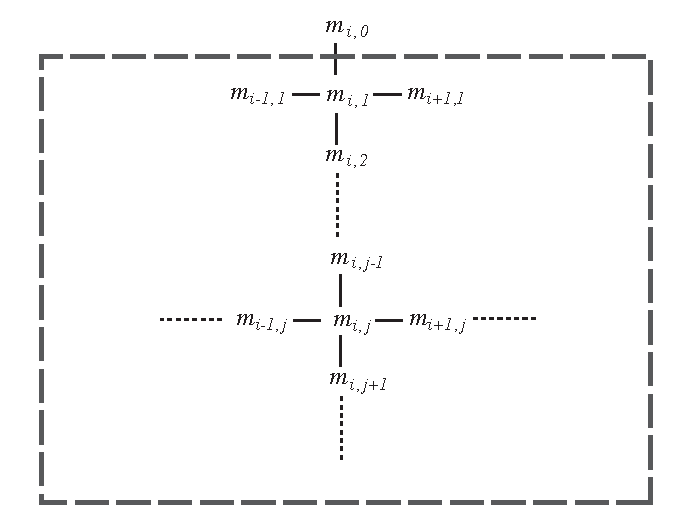
\includegraphics[width=0.75\linewidth]{./figures/ch4/laplace_stencil.pdf}
    \caption[Stencil for finite difference laplacian]{Stencil for finite difference laplacian}
  \label{fig_stencil}
\end{figure}

\begin{figure}[!ht] 
  \centering
  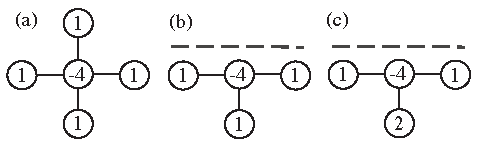
\includegraphics[width=0.75\linewidth]{./figures/ch4/molecules.pdf}
    \caption[Computational molecules]{Computational molecules for the finite difference laplacian. (a) is somewhere within the fault model. (b) is for a zero-slip condition at the top edge and (c) is a free boundary condition at the top edge.}
  \label{fig_molecules}
\end{figure}

This is problematic for a subduction zone megathrust that extends all the way to the trench. This zero-slip boundary condition is unreasonable since large slip can and should be allowed to happen at the trench. In Chapter 3 we used this boundary condition for the static slip inversion. The result is a model that does not have large amounts of motion at the trench. In order to penalize slip at the top edge of the model less harshly the stencil must be modified. We can instead require that the derivative of slip normal to the fault edge (in the dip direction, index $j$) be zero. If we approximate the first derivative by a second order accurate central difference then at the top edge we have the condition
\begin{equation}
\frac{dm_{i,1}}{dy}=m_{i,0}-m_{i,2}=0\;,
\end{equation}
where once again we assume the spacing between subfault centers is unity. This free boundary condition means that $m_{i,0}=m_{i,2}$ and yields the expression for the Laplacian at the top edge
\begin{equation}
\nabla^2m_{i,1}=\-4m_{i,1}+m_{i+1,1}+m_{i-1,1}+2m_{i,2}\;.
\end{equation}
Once again we have a 4 point stencil but the computational molecule (Figure \ref{fig_molecules}c) value for the along-dip element has changed from 1 to 2. It is a subtle modification but an important one if slip is to be allowed at the trench. Further on we will demonstrate the effect of this small change to the regularization matrix.


\subsection{Regularization and Bayesian Modeling}

The spatial Laplacian regularization matrix $\mathbf{L}_s$ and the temporal first derivative regularization one $\mathbf{L}_t$ are incorpoated into the problem as
\begin{equation}
\left(\begin{matrix}
\mathbf{G}\\
\lambda_s\mathbf{L}_s\\ 
\lambda_t\mathbf{L}_t
\end{matrix}\right)
\mathbf{m}=
\left(\begin{matrix}
\mathbf{d}\\
\mathbf{0}\\ 
\mathbf{0}
\end{matrix}\right)\;.
\end{equation}
This has the well known canonical solution \citep{menke2012}
\begin{equation}
\label{eq:solution}
\mathbf{m}^0=
(\mathbf{G}^\top\mathbf{G}+\lambda_s^2\mathbf{L}_s^\top\mathbf{L}_s+\lambda_t^2\mathbf{L}_t^\top\mathbf{L}_t)^{-1}
\mathbf{G}^\top\mathbf{d}\;.
\end{equation}
A known complication in this formulation is to objectively decide the values of the smoothing parameters $\lambda_s$ and $\lambda_t$. In Chapter 3, where we have only a spatial regularization, we employed the L-curve curvature criterion \citep{hansen2007}. However such a heuristic criterion is somewhat tricky and quite cumbersome to apply in a two dimensional parameter space. Furthermore it is somewhat unsatisfactory in that it is not grounded in a strictly objective statement about source properties. Often when perusing the literature on slip inversions it is common to find statements that indicate that for a particular study the author used his or her judgment and intuition on the physics of an earthquake to decide on a regularization parameter. This is altogether unsatisfactory, for the slip inversion there exists a probabilistic formalism that can provide objective criteria for selection of the smoothing parameters.

Following \citet{ide1996} we can write the posterior likelihood function, this is a statement about the likelihood of the inversion result, as
\begin{equation}
p(\mathbf{d}|\mathbf{m};\sigma^2)=(2\pi\sigma^2)^{-Q/2}\exp\left[-\frac{1}{2\sigma^2}\|\mathbf{d}-\mathbf{Gm}\|^2\right]\;,
\end{equation}
where $Q$ is the number of data and $\sigma^2$ is the data variance. Without any prior information maximization of this likelihood function will lead to the traditional normal equations \citep{menke2012}. If however, we consider the regularization matrices as a form of prior information we can write the following probability density functions:
\begin{eqnarray}
p(\mathbf{m}|\sigma_s^2)=(2\pi\sigma_s^2)^{-P_s/2}\|\Lambda_s\|^{1/2}\exp\left[-\frac{1}{2\sigma_s^2}\|\mathbf{L}_s\mathbf{m}\|^2\right]\;,\\
p(\mathbf{m}|\sigma_t^2)=(2\pi\sigma_t^2)^{-P_t/2}\|\Lambda_t\|^{1/2}\exp\left[-\frac{1}{2\sigma_t^2}\|\mathbf{L}_t\mathbf{m}\|^2\right]\;,
\end{eqnarray}
where $\sigma^2_s$ and $\sigma^2_t$ are hyper-parameters that represent the smoothing variance. $P_s$ and $P_t$ are the ranks of the two smoothing matrices and $\|\Lambda_s\|$ and $\|\Lambda_t\|$ are the absolute values of the product of the non-zero eigen-values of the smoothing matrices. \citet{ide1996} combined these two pdfs by simple multiplication. However \citet{fukahata2003} subsequently showed that this produces a prior pdf whose integral is not unity and thus is improper. After introducing the correct normalization, the prior pdf that combines both smoothing constraints can be expressed as
\begin{equation}
p(\mathbf{m}|\sigma_s^2,\sigma^2_t)=(2\pi)^{-M/2}\left\|\frac{1}{\sigma_s^2}\mathbf{L}_s+\frac{1}{\sigma_t^2}\mathbf{L}_t \right\|^{1/2}\exp\left[-\frac{1}{2\sigma_s^2}\|\mathbf{L}_s\mathbf{m}\|^2\right]\exp\left[-\frac{1}{2\sigma_t^2}\|\mathbf{L}_t\mathbf{m}\|^2\right]\;,
\end{equation}
where $M$ is the total number of model parameters. We can then use Bayes' theorem to define the posterior pdf of the model as
\begin{equation}
p(\mathbf{m};\sigma_s^2,\sigma_t^2,\sigma^2|\mathbf{d})=Cp(\mathbf{d}|\mathbf{m};\sigma^2)p(\mathbf{m}|\sigma_s^2,\sigma^2_t)\;,
\end{equation}
where $C$ is  a factor introduced to ensure the integral of the pdf is unity. It is, however, independent of the model parameters and hyper parameters and thus not necessary to compute. From this definition of the posterior pdf, \citet{jackson1985} showed that the optimal model $\mathbf{m}^0$ obtained from maximizing the posterior pdf is exactly the damped least squares solution of Equation \ref{eq:solution} where the ratio of the hyperparameters are actually the regularization parameters such that $\lambda_s=\sigma^2/\sigma^2_s$ and $\lambda_t=\sigma^2/\sigma^2_t$. The added benefit of taking the Bayesian approach to deriving the inverse solution is that we can use the posterior pdf to select the optimal regularization parameters.
	
\citet{akaike1980} proposed an information theory and entropy maximization based criterion, now known as the Akaike information criterion (ABIC) for selecting the adequate hyper-parameters. The parameter is obtained from the marginal likelihood as
\begin{equation}
\label{eq:abic}
\mathrm{ABIC}=-2\ln\left[\int p(\mathbf{m};\sigma_s^2,\sigma_t^2,\sigma^2|\mathbf{d})d\mathbf{m}\right]\;,
\end{equation}
thus the optimal model is the one which minimizes information loss and thus has the \textit{smallest} value of ABIC. \citet{fukahata2004} showed that the ABIC can then be expressed as
\begin{equation}
\label{eq:abic_total}
\mathrm{ABIC}(\lambda_s^2,\lambda^2_t)=Q\ln s(\mathbf{m^0})-\ln\|\lambda^2_s\mathbf{L}_s+\lambda_t^2\mathbf{L}_t\|+\ln\|\mathbf{G}^\top\mathbf{G}+\lambda_s^2\mathbf{L}_s+\lambda_t^2\mathbf{L}_t\|\,,
\end{equation}
where $s(\mathbf{m})$ is the residual
\begin{equation}
s(\mathbf{m})=\|\mathbf{d}-\mathbf{Gm}\|^2+\lambda_s^2\|\mathbf{L}_s\mathbf{m}\|+\lambda_t^2\|\mathbf{L}_t\mathbf{m}\|
\end{equation}
and the optimal model $\mathbf{m}^0$ is obtained from the damped solution in Equation \ref{eq:solution}. To use the ABIC to determine smoothing parameters you invert at several values of both smoothing parameters and compute the ABIC value for this regularization pair. Then you select as your final model the one with the smallest value of ABIC. If the smoothing is too strong then the second and third terms in Equation \ref{eq:abic_total} almost cancel each other, but the residual $s(\mathbf{m})$ is large and so is the ABIC. If the smoothing is weak then the residual is small but second term in Eqaution \ref{eq:abic_total} is large and so is the ABIC. The minimum value of ABIC is somewhere between these two extremes and in a sense represents the tradeoff between he residual $s(\mathbf{m})$ and the condition number of the regularized matrix \citep{ide2007}. This approach is a combination of traditional inversion with Bayesian modeling and has been employed by several researchers for kinematic inversions. It has been used, for example, to study the $M_w$ 6.0 Kobe earthquake \citep{sekiguchi2000} the $M_w$7.6 Chi-Chi earthquake \citep{wu2001} and the $M_w$9.0 Tohoku-oki event \citep{yoshida2011}.
A benefit of this Bayesian framework is that if the covariance matrix of the data, $\mathbf{C_d}$ is known then we can compute the covariance of the model parameters as \citep{yabuki1992,ide2007}
\begin{equation}
\mathbf{C}_m=\sigma^2(\mathbf{G}^\top\mathbf{C}_d\mathbf{G}+\lambda_s^2\mathbf{L}_s^\top\mathbf{L}_s+\mathbf{L}_t^\top\mathbf{L}_t)^{-1}\;,
\end{equation}
where
\begin{equation}
\sigma^2=\frac{s(\mathbf{m}^0)}{Q}\;.
\end{equation}
This allows us to make statistical statements about the reliability of a given solution, something that is tricky for traditional high order Tikhonov regularized inverse solutions \citep{aster2013}.


\section{An example with seismogeodetic data, the $M_w9$ Tohoku-oki earthquake}

As discussed in Section \ref{sec_backgr}, for inversion with regional data there are limitations to using just strong motion or high-rate GPS data. We will now demonstrate the performance of the seismogeodetic data for a kinematic inversion of the Tohoku-oki event and argue that it produces a more robust solution than with either data set alone. We select 20 stations from the Kalman filtered dataset described in Chapter 2 and invert the three component displacements and velocities for a total of 120 waveforms. As mentioned in the previous section, displacement based inversions will be biased but he predominance of longer period data while velocity based inversions will provide higher frequency information. In order to obtain a model that is suitable across as broad a frequency range as possible we invert both data types. The stations are selected to provide adequate coverage of the rupture area (Figure \ref{fig_kinmap}) while also taking into account the site conditions. For a static slip inversion the site response is not of great importance, so long as there is no ground failure, the coseismic offset will be largely independent of site response. However many of the GPS/accelerometer pairs belong to the Knet strong motion network which can often have significant site response \citep{tsuda2006}. Luckily, for every strong motion station in Japan there exists a soil profile (http://www.kyoshin.bosai.go.jp/). We ensured that all the selected sites for the inversion had a $v_{s30}$ larger than 500m/s in order to avoid any site effects contaminating the inversion results. Of the 20 sites selected 6 belong to the KiKnet network and 14 to the Knet network.

\begin{figure}[!ht] 
  \centering
  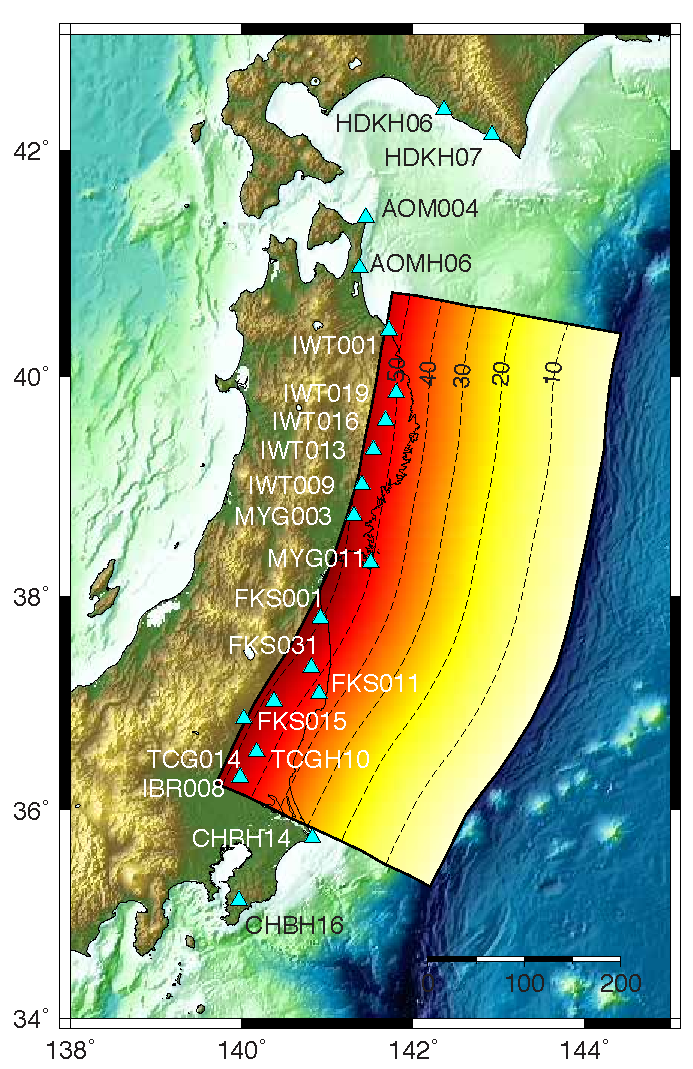
\includegraphics[width=0.55\linewidth]{./figures/ch4/kinmap.pdf}
    \caption[Station distribution for kinematic inversion]{Map of 20 stations used in the seismogeodetic slip inversion. The slab geometry used for the inversion is the same as that of Chapter 3 from \citet{hayes2012}. The contours are depth to the slab in kilometers.}
  \label{fig_kinmap}
\end{figure}

The fault model (Figure \ref{fig_kinmap}) is the same as that of Chapter 3. It is a discretized version of the Slab 1.0 model of \citep{hayes2012}. It consists of 21 along strike and 9 down-dip 25$\times$25km sub-faults (189 in total). We use a 1D layered model calibrated for Japan. The model, shown in Table \ref{tb_toku_model}, is used for automated computation of CMT's with long period data \citep{fukuyama1998,tsuruoka2009}. For the Green functions calculation we use the fk code provided by \citep{zhu2002} and compute GFs for every subfault/station pair from 0 to 0.5Hz. The data are lowpass filtered to 0.5Hz to match the GFs. We use triangular source-time functions with a 10s rise time. This choice is rather arbitrary and this is perhaps the most ad-hoc parameter in the process. However, a rise time of 10s allows for the rupture front to traverse the subfault at a sensible velocity and is in broad agreement with the source-time function scaling laws of \citep{tanioka1997}. The maximum rupture velocity allowed is 3.5km/s which corresponds to 0.8 times the shear wave speed ($0.8\beta$) of the fastest layer spanned by the slab model (layer 4). We then allow slip on 20 subsequent 50\% overlapping triangle source time functions with equal rise time (10s) yielding a total of 7560 model parameters. This parametrization allows each subfault to slip for a total of 105s. Recall that this does not mean that rupture speed is forced to 0.8$\beta$, rather that this is the fastest possible velocity in the model. In fact choosing instead a maximum rupture velocity of $0.9\beta$ or 4km/s has little effect on the inversion results. Subsequently, the inversion is run using a NNLS solver to enforce positivity. To sample a large portion of the parameter space spanned by $\lambda_s$ and $\lambda_t$ we first invert on a coarse gird of smoothing parameters (between $10^{-5}$ and $10^2$). A total of 64 different $(\lambda_s,\lambda_t)$ pairs are used. We then refine the smoothing parameter grid twice more around the minimum ABIC inversion result to define the smoothing parameters that are used for final inversion. Furthermore, because the displacement time series are significantly larger in magnitude than the velocity time series (peak displacement is several meters, while peak velocity is tens of centimeters per second) it is necessary to weigh the data appropriately. We take the ratio of the norms of the displacement and velocity time series (a value of 36.06) and apply that value to the velocity time series. In this way we ensure that the inversion penalizes misfit to the displacements and velocities equally. If this weight is not applied the inversion will preferentially fit the displacement data.

\begin{table}
\caption{Velocity model for the Tohoku-oki kinematic inversion}
\label{tb_toku_model}
\begin{tabular}{l r r r r r r}
\hline
Layer & $v_p$ & $v_s$ &Density&Thickness&$Q_p$&$Q_s$\\
 & (km/s) &( km/s) & (kg/m$^{3}$) & (km) &  &\\
\hline
1 & 5.50 & 3.14 & 2.30 & 3.0 & 600 & 300\\
2 & 6.00 & 3.55 & 2.40 & 15.0 & 600 & 300\\
3 & 6.70 & 3.83 & 2.80 & 15.0 & 600 & 300\\
4 & 7.80 & 4.46 & 3.20 & 67.0 & 600 & 300\\
Half-space & 8.00 & 4.57 & 3.30 & $\infty$ & 600 & 300\\
\hline
\end{tabular}
\end{table}

\subsection{Kinematic Inversion Results}
Figure \ref{fig_ABIC} shows the values of the ABIC for 100 inversions with different levels of regularization. As discussed we select the preferred values of $\lambda_s$ and $\lambda_t$ from the global minimum of that plot. The total slip from this preferred kinematic inversion is shown in Figure \ref{fig_totalslip}a and has a peak slip value of 52m on the shallowest subfault. Large slip, in excess of 20m happens on an asperity of about 300x150km up dip of the hypocenter at depths shallower than 20km. Slip at depth tapers of quickly but there isa till a large area of roughly 200x100km with more than 5-20m of slip extending from a depth of about 50km up dip to the hypocenter. Figure\ref{fig_totalslip}b is the source time function for the preferred model. Moment rate begins very slowly between 0 and 20s but increases sharply to its peak at 75s. Afterwards it decreases smoothly, the total duration of moment release is around 185s for this model. The total moment is $4.9\times10^{22}\textrm{N-m}$ or $M_w9.06$.
\begin{figure}[!ht] 
  \centering
  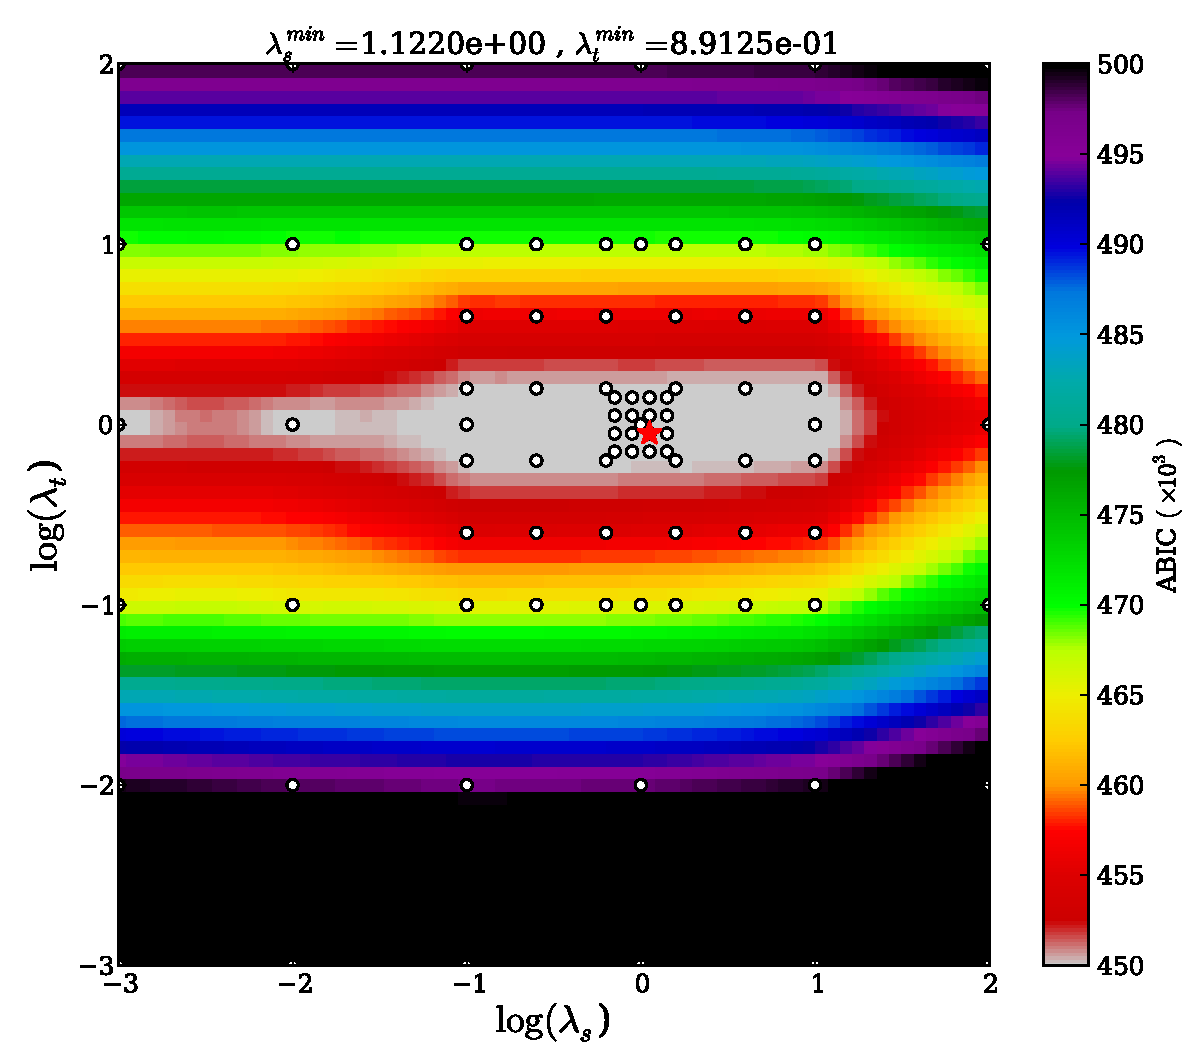
\includegraphics[width=0.85\linewidth]{./figures/ch4/ABIC.pdf}
    \caption[ABIC values for kinematic inversion]{Values of ABIC for the kinematic inversion. The white dots are the values used for 100 inversions to determine the minimum ABIC. The red star is the minimum.}
  \label{fig_ABIC}
\end{figure}

\begin{figure}[!ht] 
  \centering
  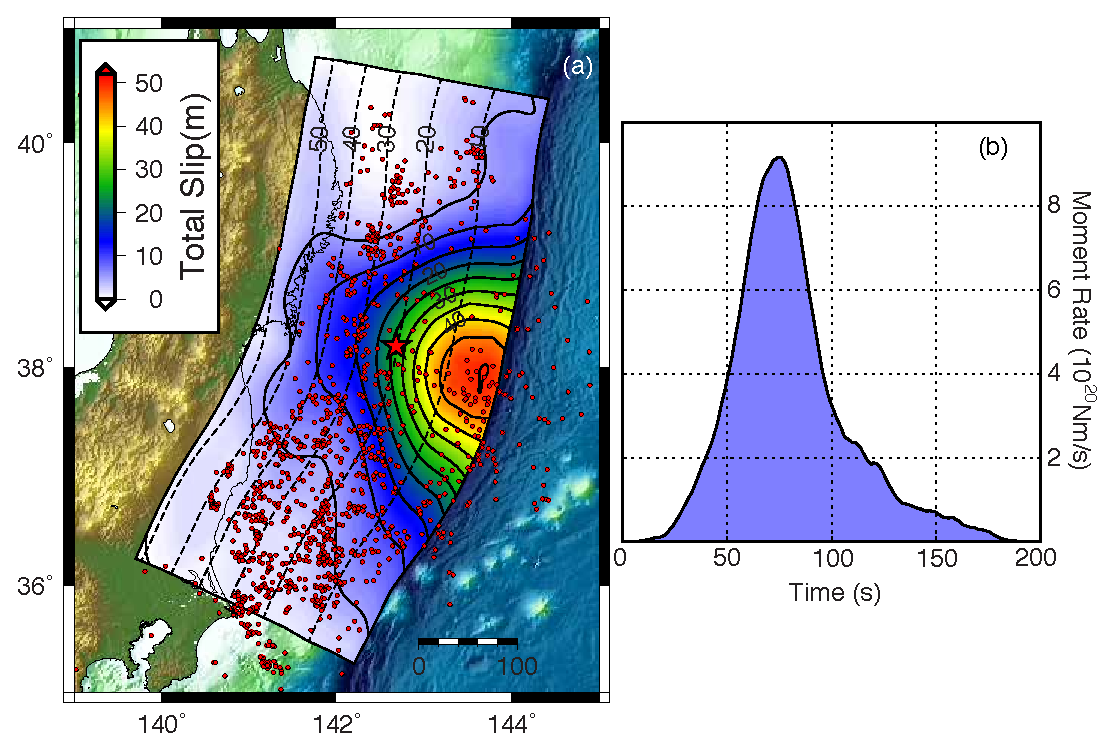
\includegraphics[width=0.99\linewidth]{./figures/ch4/total_slip_moment_rate.pdf}
    \caption[Kinematic inversion results]{(a) Total slip from the kinematic inversion, peak slip is 52m. The red star is the epicenter and the red circles are two weeks of aftershocks from the NIED catalogue. Slip is contoured every 10m and the slab depths are contoured every 10km in dotted lines. (b) The source time function for the kinematic model. }
  \label{fig_totalslip}
\end{figure}

The fits to the data are shown in Figure \ref{fig_dispfits} for the displacement time series and in Figure \ref{fig_velfits} for the velocity time series. Variance reduction is high for the displacements (90\%) and somewhat lower (77\%) for the velocity time series.  The displacement times rise are mostly well modeled, the notable exception is in the two northern stations in Hokkaido island HDKH06 and HDKH07 were the amplitude of surface waves arriving between 200 and 300s are under estimated. This is also true for the velocity time series. However we also observe in the velocity time series an underestimation of the higher frequencies. This is obvious for example for stations TCGH10 and IBR008 both in the Kanto region and also for the northern stations in Aomori prefecture (AOM004 and AOMG06) and in Hokkaido island (HDKH06 and 07)

\begin{figure}[!ht] 
  \centering
  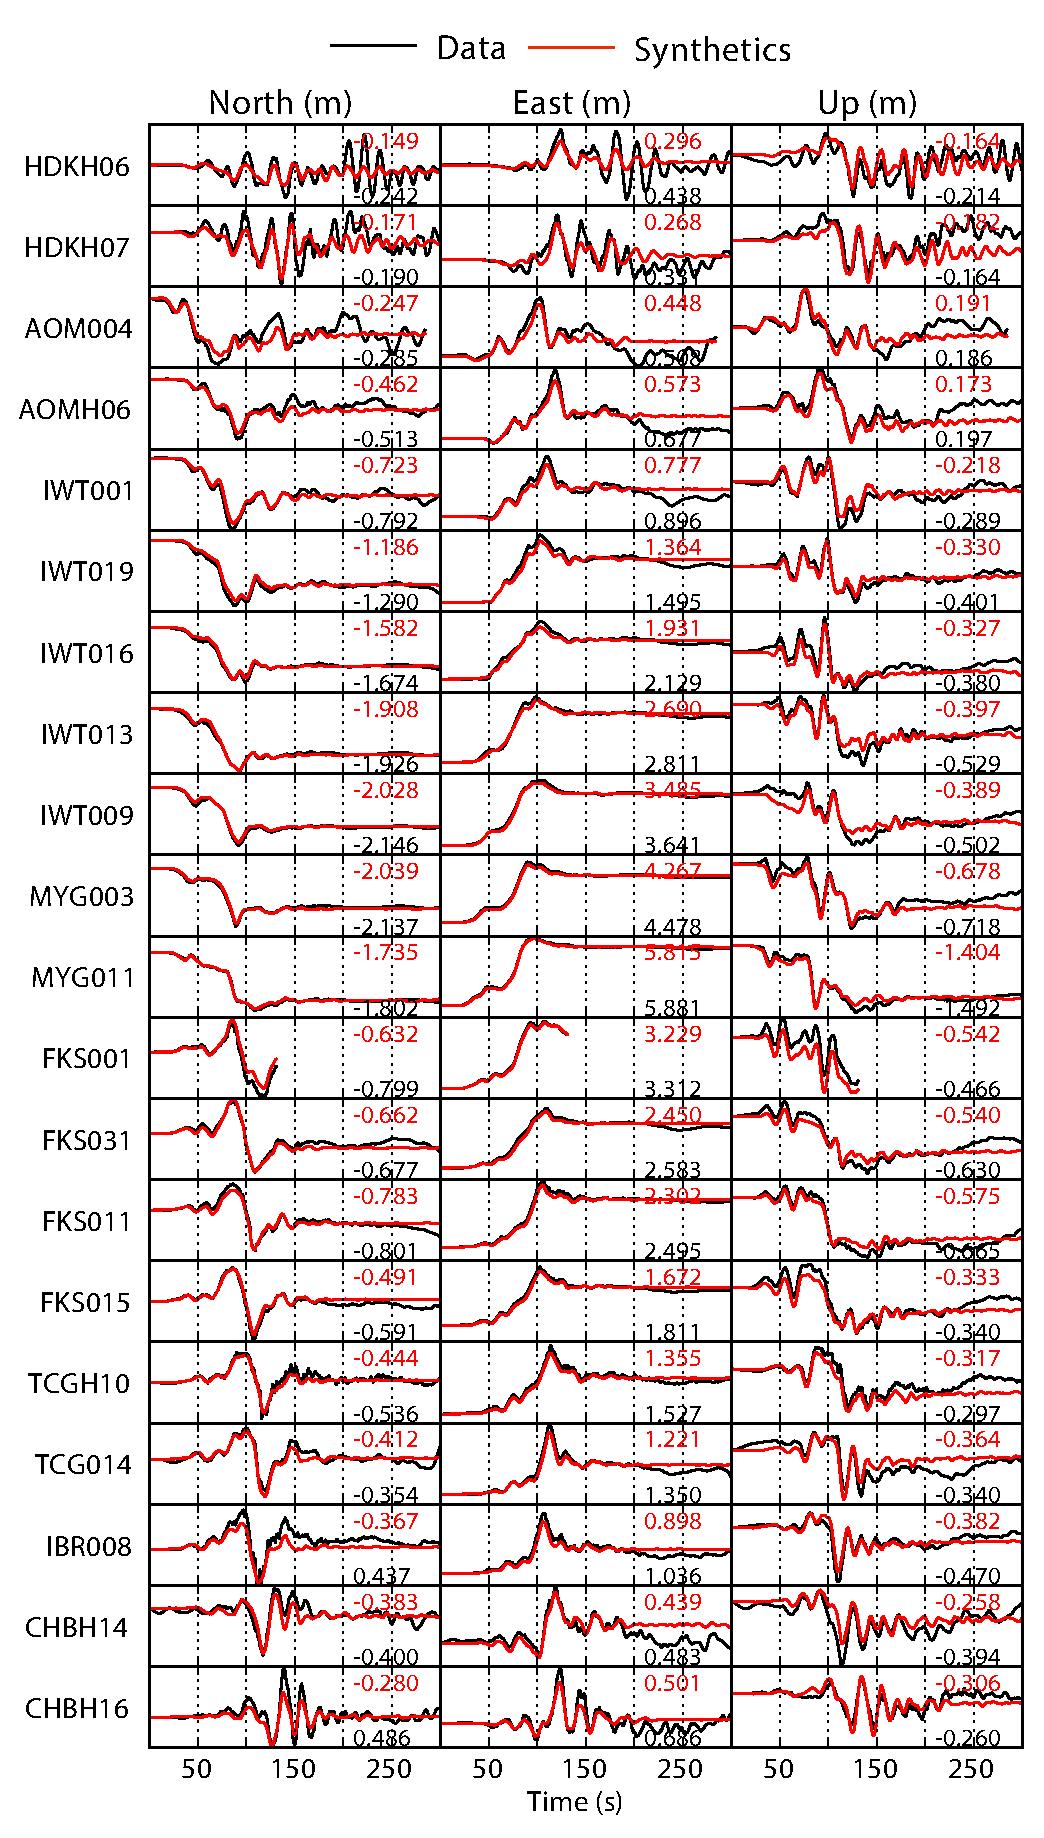
\includegraphics[width=0.72\linewidth]{./figures/ch4/disp_data_vs_synthetics}
    \caption[Data fits No. 1 for the kinematic inversion]{Comparison between observed (black) and synthetic (red) 3-component displacement time series. The stations are sorted by latitude from north to south (see Figure \ref{fig_kinmap}). The numbers next to the time series represent the value of peak displacement}
  \label{fig_dispfits}
\end{figure}

\begin{figure}[!ht] 
  \centering
  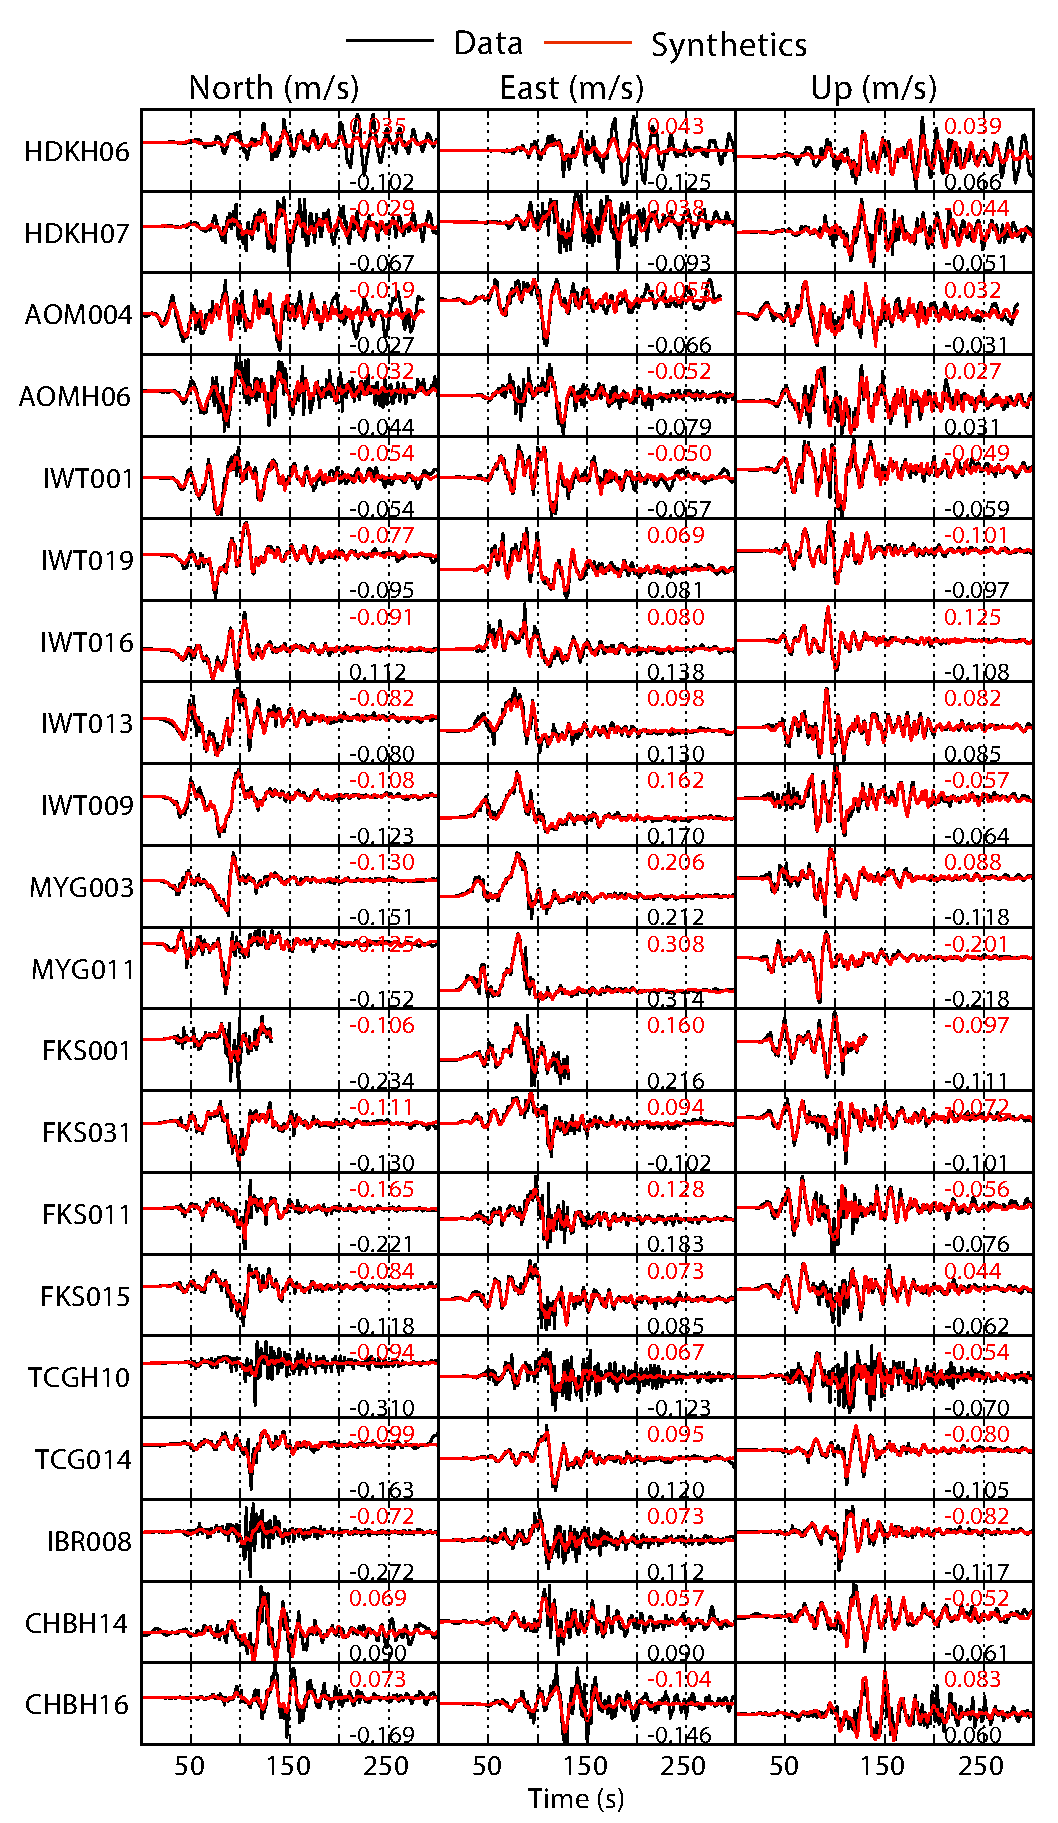
\includegraphics[width=0.72\linewidth]{./figures/ch4/vel_data_vs_synthetics}
    \caption[Data fits No. 2 for the kinematic inversion]{Comparison between observed (black) and synthetic (red) 3-component velocity time series. The stations are sorted by latitude from north to south (see Figure \ref{fig_kinmap}). The numbers next to the time series represent the value of peak velocity}
  \label{fig_velfits}
\end{figure}

The time evolution of slip can be seen in Figure \ref{fig_snapshots} where we present 10s snapshots of 160s of rupture. We have include 3 pseudo-rupture fronts in the plot that show the approximate distance a rupture from traveling at 1.5, 2.5 and 3.5km/s would have traveled. In agreement with the source time function of Figure \ref{fig_totalslip}b, the rupture starts slowly, propagating both up and down-dip. At around 30s the rupture accelerates up dip and expands along strike rapidly reaching peak slip at around 70s. Up dip there is slip of at least 10m on a segment of about 350km in length. Down dip the behavior is very different. There is an initial slip pulse that propagates down from the hypocenter at around 2.5km/s until about 50s and to about 45km depth. This is followed by a second pulse of deep slip starting at about 60s that propagates down from the epicenter and then laterally, very quickly, mostly along-strike to the south. There is very little slip at depths larger than 50km.

\begin{figure}[!ht] 
  \centering
  \includegraphics[width=0.95\linewidth]{./figures/ch4/snapshots_10s.pdf}
    \caption[Model snapshots]{Snapshots of slip propagation in 10s increments, the red star is the epicenter and the black contour is the 1m of slip contour. The three brown concentric circles represent pseudo rupture fronts propagating at 1.5, 2.5 and 3.5 km/s respectively.}
  \label{fig_snapshots}
\end{figure}

Another way to examine the time dependent behavior of rupture is to study the individual source time functions (STFs) of each subfault. Figure \ref{fig_tiles} illustrates precisely this. Plotted is the moment rate for every subfault with their respective 90\% confidence intervals (CIs). The white lines indicate the lower bounds of the 90\% CIs and the grey hatched areas the upper bound of the CI. The STFs are colored by pseudo-rupture velocity. This coloring serves the same purpose as the pseudo rupture fronts in Figure \ref{fig_snapshots}. It indicates how fast a rupture front would have to travel to each that subfault at a particular instant in time. They are a visual aid to understand the changes in rupture speed in the model. We observe the same pattern as in Figure \ref{fig_snapshots}. Rupture begins slowly at first but accelerates up-dip reaching the the shallowest portions of the model at a pseudo velocity of around 3km/s and spreading along strike. Down dip there seem to be at least two pulses of slip, the second one indicating a very low initial rupture speed down dip from the hypocenter that spreads laterally quite quickly. The CI are a guide to avoid over-interpretation of the STFs. Another feature present in this plot is the duration of the source time functions. Up dip of the hypocenter rupture durations are long, usually 50s or longer while down dip the two pulses of slip are closer to 20s each. This makes the up dip STFs very smooth and the deeper ones very peaked suggesting a a depth dependence of the physical properties of the source.

%\begin{sidewaysfigure}[!ht]
 %   \includegraphics[width=0.99\linewidth]{./figures/ch4/tiles_small.pdf}
  %  \caption[Subfault source-time functions]{Subfault source-time functions (STFs). The 90\% confidence intervals are indicated by the white line and the solid grey hatched area. The coloring under the STFs represents the pseudo rupture velocity. The red star indicates the hypocenter. All STFs are plotted at the same scale.}
 %   \label{fig_tiles}
%\end{sidewaysfigure}

\subsection{The Effect of Spatial Regularization}
In Section \ref{sec:regu} we discussed modifications to the Laplacian smoothing kernel used for regularization. We argued that the traditional 5 point stencil would place a large penalty on slip at the trench and suggested a modification. A brief demonstration shows this is indeed the case.  The model of Figures \ref{fig_totalslip} and \ref{fig_tiles} shows large slip and moment release in the shallowest parts of the fault. However, if we apply the traditional locked boundary condition we obtain the model shown in Figure \ref{fig_total_locked}. Total slip in this model is marginally larger (53m) than out preferred model while total moment is almost identical ($4.73\times10^{22}Nm$ or $Mw9.05$). However, peak slip is now at around 12km depth and slip at the trench is significantly smaller (25m or less) than that of the preferred model. As discussed, large slip is discouraged with the traditional Laplacian stencil.

\begin{figure}[!ht] 
  \centering
  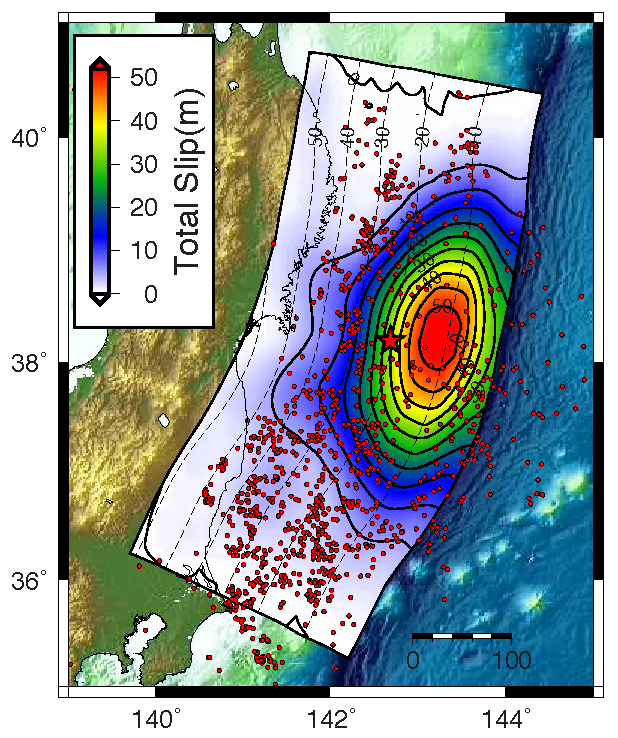
\includegraphics[width=0.6\linewidth]{./figures/ch4/total_slip_locked.pdf}
    \caption[Totals lip with a locked boundary condition]{Total slip from the kinematic inversion with a locked boundary condition at the trench, peak slip is 53m. The red star is the epicenter and the red circles are two weeks of aftershocks from the NIED catalogue. Slip is contoured every 10m and the slab depths are contoured every 10km in dotted lines. }
  \label{fig_total_locked}
\end{figure}


\subsection{The Displacement-only Solution}

We inverted for a kinematic model using only the seismogeodetic displacements. The total slip results are shown in Figure \ref{fig_total_disponly}a. Slip is considerably larger (71m at the trench) while moment is $5.32\times10^{19}$ or $M_w9.08$ only slightly larger than the combined displacement and velocity solution. The peak moment rate (Figure \ref{fig_total_disponly}b is larger at $13\times10^{20} Nm/s$, almost 50\% more than for the combined solution. Furthermore, while the duration of rupture is similar (180s) peak moment release happens earlier (65s) than in the combined solution; the displacement only solution has very little moment after 140s. This is best seen in Figure \ref{fig_stf_compare} where the two STFs are plotted for comparison. The models are similar up to 50s, then the displacement-only model accelerates its moment release quickly to its peak, while the combined model shows a smoother evolution to peak moment release. After the peak, the ramp-down is similar for both events, but after 100s the displacement only model tapers off to low moment rates very quickly while the joint model continues to have significant moment release during the ramp-down. The longer source time function of the joint model is supported by almost all tele seismic inversions \citep{shao2011}, the low frequency back projection studies \citep{kiser2012} and hybrid back-projection models that include depth phases \citep{yagi2012}.


\begin{figure}[!ht] 
  \centering
  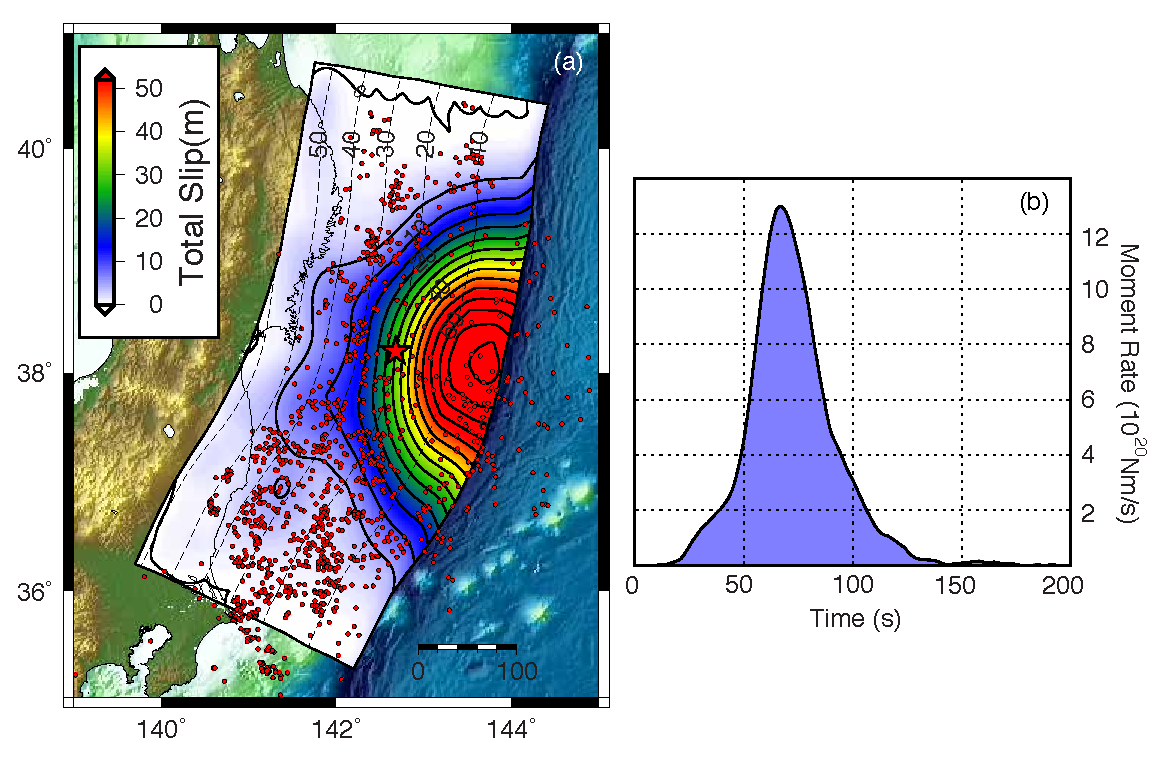
\includegraphics[width=0.9\linewidth]{./figures/ch4/total_slip_moment_rate_disp_only.pdf}
    \caption[Total slip with seismogeodetic displacements only]{Total slip from the kinematic inversion with only seismogeodetic displacements, peak slip is 71m. We've retained the color scheme from Figure \ref{fig_totalslip} to facilitate comparisons. The red star is the epicenter and the red circles are two weeks of aftershocks from the NIED catalogue. Slip is contoured every 10m and the slab depths are contoured every 10km in dotted lines. }
  \label{fig_total_disponly}
\end{figure}

\begin{figure}[!ht] 
  \centering
  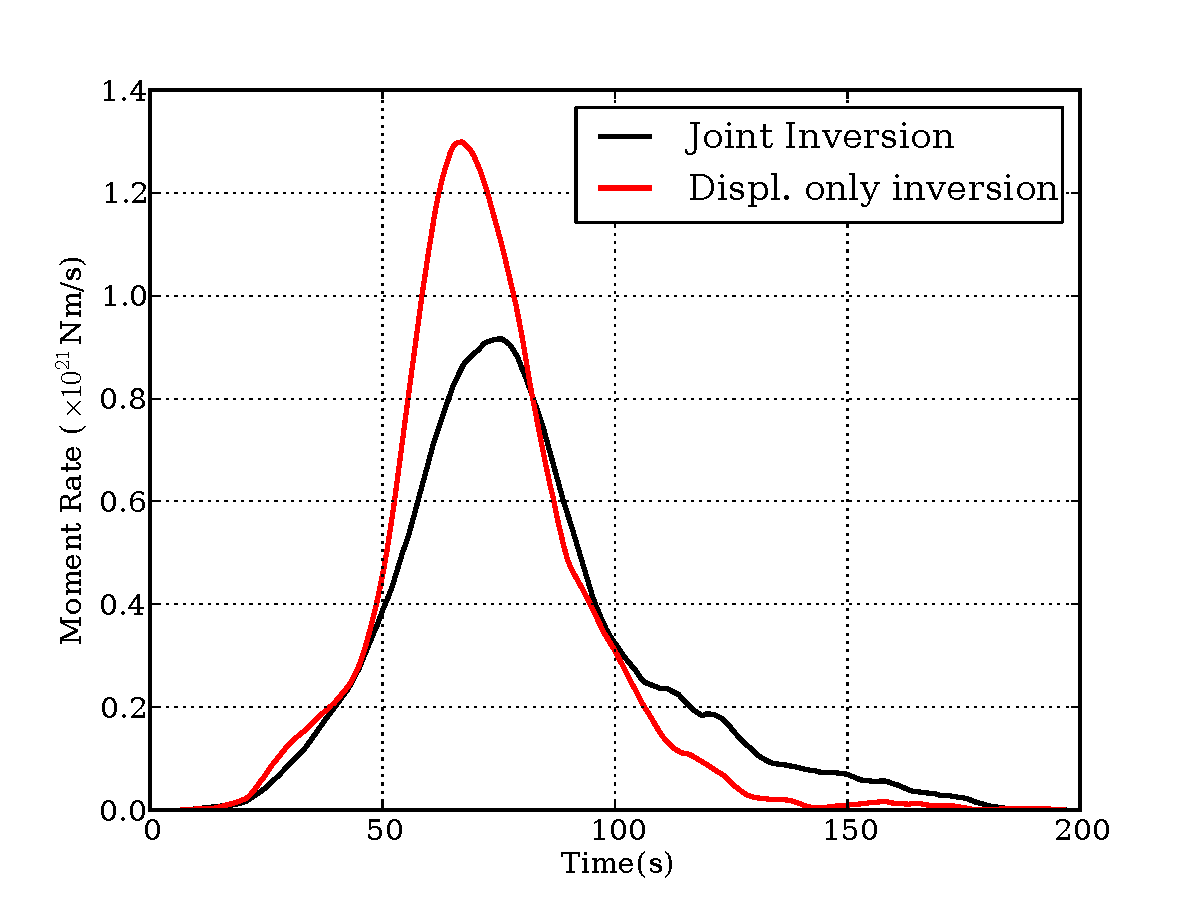
\includegraphics[width=0.72\linewidth]{./figures/ch4/source_TF_compare.pdf}
    \caption[Source time function comparisons]{Comparison between the source time functions of the joint inversion of displacement and velocity data and the displacement-only solution}
  \label{fig_stf_compare}
\end{figure}

Another view of the differences between the displacement-only and joint solutions can be seen in Figure \ref{fig_tiles_disp} . Here we've plotted ocher more the individual source-time functions for each subfault. Significant differences can be seen. Notice that the scale is different between Figures \ref{fig_tiles} and \ref{fig_tiles_disp}. Peak moment rate is $3\times10^{19}Nm/s$ in the joint solution and $5\times10^{19}Nm/s$ in the displacement-only model. Broadly speaking the shapes of the STFs are similar but, in this solution, they are smoother than in the joint solution. There also seem to be some inconstancies in the timing of rupture. The shallow subfaults (row No.1) have a mixture of fast rupture along strike that has not been reported in other results. Specifically the subfaults at positions 4-6 and 14-17 favor a fast rupture of 3+km/s while the central one with the largest moment (Nos. 8-12) favor a slower rupture closer to 2.3 km/s. This behavior of subfaults favoring fast rupture surrounded by slower rupture subfaults is also seen in rows 4 and 5. Down-dip moment is also significantly smaller in the displacement only solution.

\begin{sidewaysfigure}[!ht]
    \includegraphics[width=21cm,height=7cm]{./figures/ch4/tiles_disp_small.pdf}
    \caption[Subfault source-time functions]{Subfault source-time functions (STFs) for the displacement-only solution. The 90\% confidence intervals are indicated by the white line and the solid grey hatched area. The coloring under the STFs represents the pseudo rupture velocity. The red star indicates the hypocenter. All STFs are plotted at the same scale.}
    \label{fig_tiles_disp}
\end{sidewaysfigure}

These observations, together with the longer total source time function of the joint model suggest that the net effect of including the velocity time series is that they provide improved control on the timing of rupture. In this case, this has the secondary effect of reducing the peak slip from 71 to 52m with a minimal reduction in total moment. The displacement only solution from the Kalman filter still has significant detail and some of the broad features agree with the combined solution. This is important; models derived from low pass filtered GPS data alone \citep{yue2011} show much less detail in the subfault source-time functions. Furthermore they are fairly insensitive to rupture velocity. \citet{yue2011} showed that data fits to the GPS data were mostly unchanged when assuming maximum rupture velocities anywhere between 1.5 and 3km/s and even higher. This lead them to prefer a model with a maximum rupture speed of 1.5 km/s which we now know from back projection studies \citep{wang2011bp,kiser2012} is far too slow for the whole rupture. In fact if we choose such a slow rupture velocity in our inversions the fits to the velocity waveforms are severely degraded. Again, the velocity data provide improved control on the timing of slip, but we recognize that the seismogeodtic displacement only results still provide a significant improvement over GPS-only solutions.

\subsection{Implications of the Model}

We have discussed at length the effect of adding the seismogeodetic time series to the inversion procedure; the provide better control on the timing of rupture. It is important as well to discuss the frequency limits of our inversion results which rely on data low pass filtered at 0.5Hz. Figure \ref{fig_coherence} shows the coherence between data and synthetics for the preferred model. Coherence is typically high at periods longer than 7-8s and lower at higher frequencies. However we still see bands of high coherence at higher frequencies in both the displacement and velocity data. We attempted to invert data low pass filtered at 1Hz and found in general very low coherence at frequencies higher than 0.5Hz. It is quite likely that the degradation in the fits to the data at periods shorter than 7-8s is due to the large spatial discretization we have chosen as well as un-modeled Earth structure \citep{graves2001,wald2001}. One area of immediate improvement would be to use GFs for more realistic Earth models. 

\begin{figure}[!ht] 
  \centering
  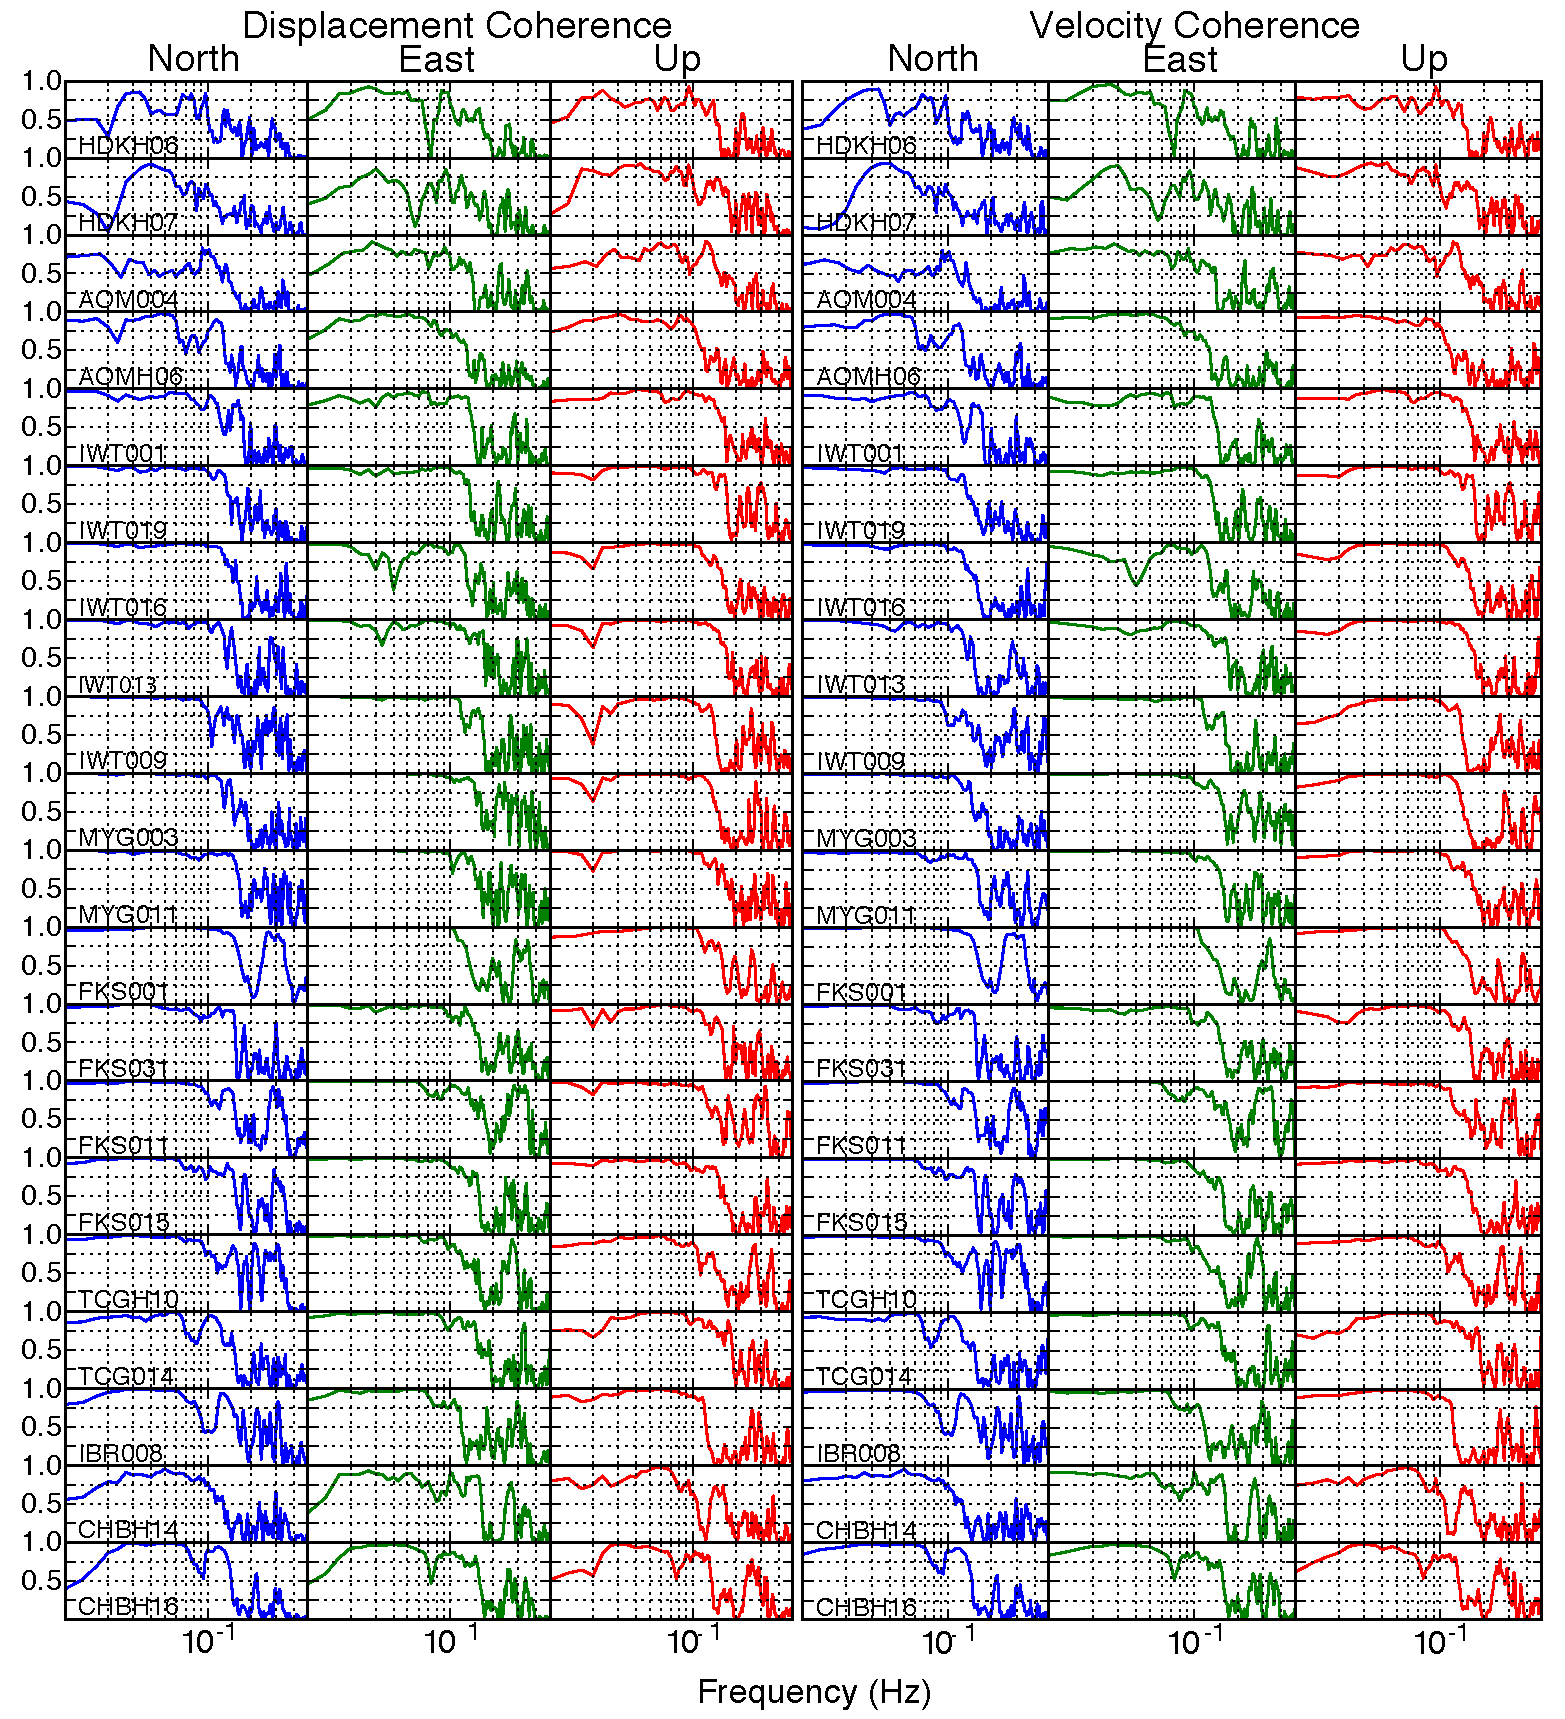
\includegraphics[width=0.99\linewidth]{./figures/ch4/all_coherence.pdf}
    \caption[Coherence plots]{Coherence between observed and synthetic data for the joint inversion results. The stations are sorted from north to south (Figure \ref{fig_kinmap})}
  \label{fig_coherence}
\end{figure}

However, the elevated coherence at higher frequencies does seem to indicate that inversion of seismogeodetic data is capable of modeling a broadband set of source features. Typically, back projection studies are conducted at frequencies higher than 0.5-1.0 Hz. For Tohoku this was the case for the earlier studies \citep{wang2011bp,koper2011}. While the model results shown here broadly agree with those high frequency source images, it is difficult to defend such an assertion given the differing frequency ranges over which they image the source. There have been however, low period back projection studies, particularly \citet{kiser2012} (0.05-0.5Hz) and \citet{yagi2012} (0.1-0.5Hz) that we can compare our results against. The comparison shows good agreement, the hybrid back projection of \citet{yagi2012} shows an initial up dip rupture speed of 3km/s which is similar to what we find. Down dip they image a fast (4km/s) pulse of slip followed by a slower one (1.5km/s) that then expands along strike, mostly to the south. Meanwhile \citet{kiser2012} do not resolve the initial up-dip slip but of see the slow down dip pulse (0.8km/s) which then rapidly expands laterally to the south at (3.4km/s). We see similar features in our preferred model (Figures \ref{fig_snapshots} and \ref{fig_tiles}). 

The model is also in agreement with longer period observations. Particularly with the tele-seismic model of \citet{shao2011} which uses wavelet analysis. Such a model assigns equal weights to all frequency components and is not biased by short period body waves or long period surface waves, and is thus easier to compare against. The total slip is similar as is the time evolution of rupture. Additionally we are able to model large amounts of slip in the shallowest portion of the model in agreement with seafloor geodetic observations and repeat bathimetry \citep{fujiwara2011,sato2011}. This suggests that the seismogeodetic inversion with displacement and velocity data provides a broadband image of the source, we can capture both the high frequency features of rupture and the longer period detail as well.

The preferred kinematic model shown in Figures \ref{fig_totalslip} and \ref{fig_tiles} can be interpreted under the framework of the depth varying properties of subduction zone megathrusts \citep{lay2012}. The megathrust can be divided into 4 domains, domain A which extends from the trench to around 10-15km and experiences either aseismic stable sliding or large coseismic rupture during tsunami events. Domain B then extends down to around 35km and has large total slip while being relatively depleted of coherent high frequency radiation. Domain C extends from there down to 55km depth and usually has reduced amounts of slip but higher content of short period radiation. Domain D is the transition to stable sliding where slow slip and tremor tend to occur. This is a conceptual model and there is significant variability worldwide. The difference between domains B and C lies in that in Domain B are the shallow, large asperities while deeper in domain C there are only smaller asperities surrounded by conditionally stable material.

The reason for these differences is varied and disputed. Variations in geometry, mineral phases, fault roughness, pore fluids, thermodynamic conditions and rock types likely all contribute \citep{heuret2011}. However the conceptual model of \citep{lay2012} indicates that whatever the cause, there should be observable differences in the behavior of the fault at depth and the Tohoku event ruptured the three seimogenic domains (A-C). From our source model we can make some interesting observations about the rupture. It nucleates at 21km depth in domain B and after a modest initial phase produces large amounts of moment release in domain A in a steady smooth fashion. There is evidence of a tsunami event, the 1896 Sanriku earthquake which ruptured the shallowest part of the northern half of the Tohoku-oki source region with about 6m of slip \citep{tanioka1996}. This is significantly smaller than the large slip (50m) we observe in our results. This indicates that the shallow domain A section must be capable of strain accumulation, if only slowly, and is not simply slipping aseismically. It is also possible that dynamic weakening can change the rate and state properties of domain A \citep{noda2013} such that it can participate in coseismic rupture. This means that under certain conditions rupture from below can instigate shear failure in the usually creeping shallow section of the mega-thrust.

If the megathrust properties vary with depth then the nature of rupture should as well \citep{lay2012}. Indeed, we can observe such behavior in our model. Figure \ref{fig_stfpsd}a shows the normalized multi-taper power spectral densities of the slip rate functions from Figure \ref{fig_tiles}. We can see a marked difference between the shallow and deep slip rate spectra. Figure \ref{fig_stfpsd}b shows the spectra stacked by the along-dip row number. It is clear that the shallow sub faults are depleted in short-period energy. High frequency radiation increases with depth. The confidence intervals on the source-time functions (Figure \ref{fig_tiles}) imply that this interpretation must be taken with caution. Particularly for the deeper sub faults which small moment release. However, the slip model we've derived agrees well with modern conceptual frameworks of megathrust ruptures. The long, smooth, source time functions with large slip on the shallow parts of the fault could be related to slip on a low friction fault and fast, sharp slip of short duration at depth is likely related to brittle failure on a high friction fault \citep{kanamori2004}. Indeed, initial results from deep cores obtained by the JFast drilling project suggest a very low coefficient of friction in the shallow megathrust \citep{fulton2013}. The source models derived from seismogeodetic data are useful not only for rapid hazards applications (as we'll discuss below) but are also suitable for detailed analyses of the earthquake source.

\begin{figure}[!ht] 
  \centering
  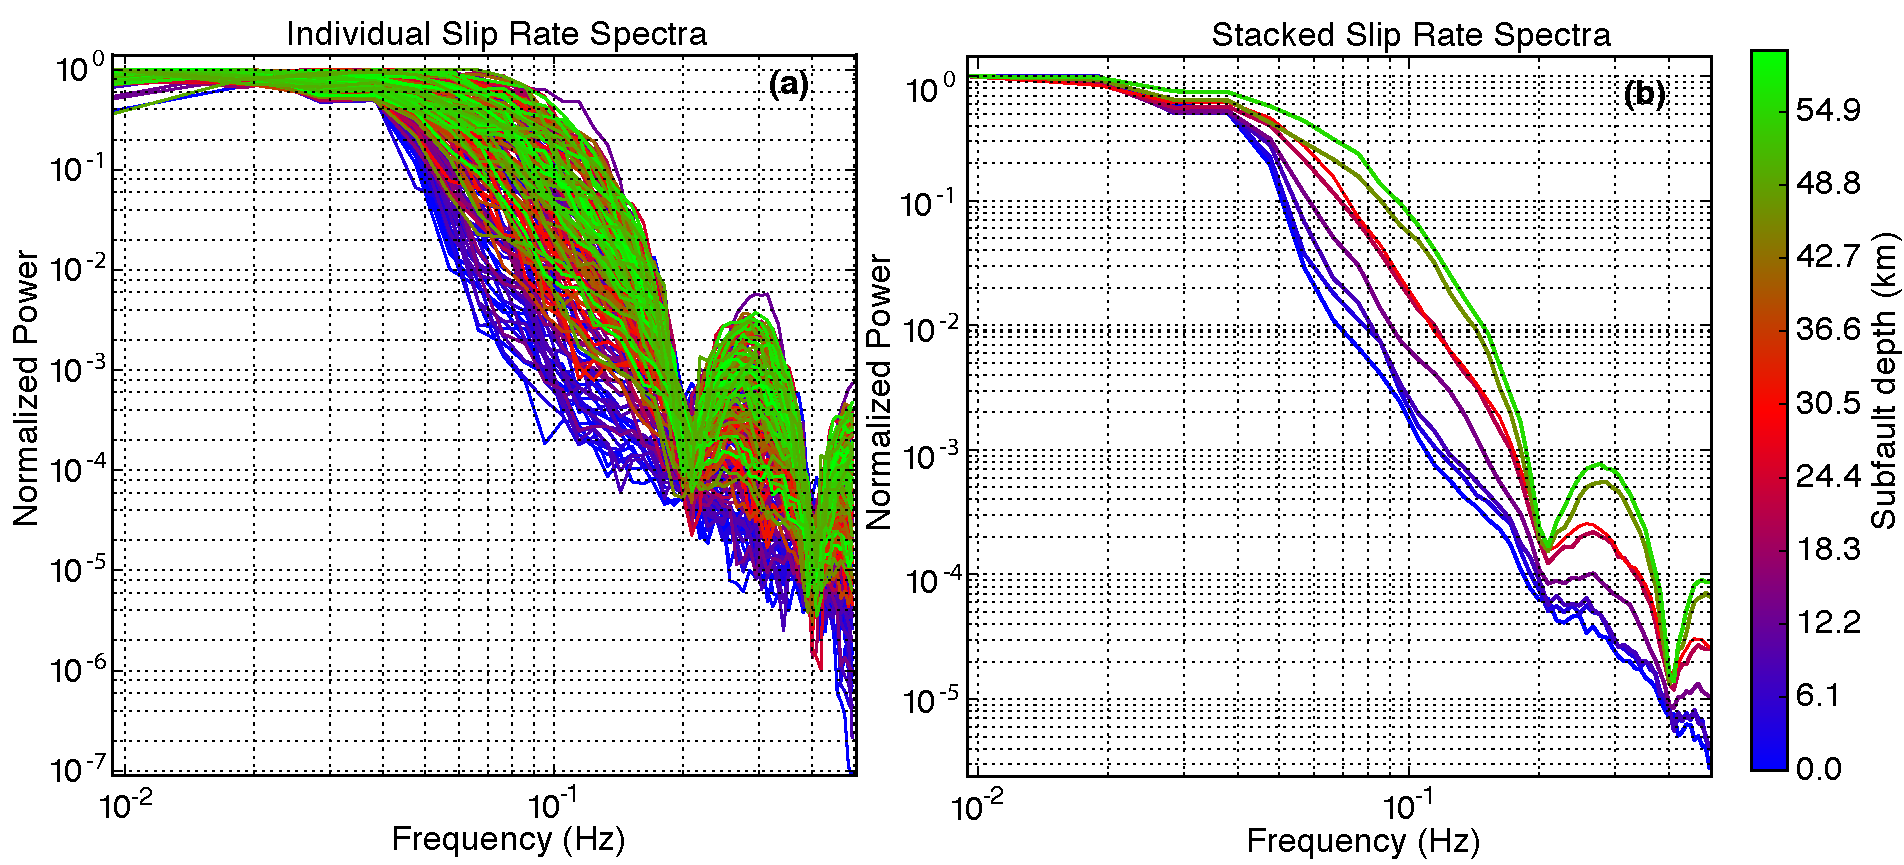
\includegraphics[width=0.99\linewidth]{./figures/ch4/stf_all.pdf}
    \caption[Source time function spectra]{(a)Normalized power spectral densities for the slip rate functions of all sub faults shown in Figure \ref{fig_tiles}.(b) Normalized stacked PSDs for the sub fault source time functions. The spectra are stacked per down-dip row of the model and the color corresponds to their average depth.}
  \label{fig_stfpsd}
\end{figure}

\subsection{Suitability for Rapid Implementation}

The issues facing real-time or rapid implementation of a kinematic inversion algorithm like the one discussed in this chapter are similar to those highlighted for the static case in Chapter 3. The style of faulting needs to be independently determined, this is paramount to selecting an adequate fault geometry for the slip inversion. The \textit{fast}CMT moment tensor solution can be used; once thrust faulting is ascertained and its location placed close to the megathrust a precomputed slab model such as Slab 1.0 \citep{hayes2012} can be employed. Recall that the first limitation facing implementation of a slip inversion with regional data is the unreliability of strong motion data at long periods and the slow sampling rates and high noise levels of GPS data. The seismogeodetic approach overcomes this and allows the seismologist to access the whole suite of source modeling ethos discussed in Section \ref{sec_backgr}. Non-linear inversions or wavelet based techniques can be utilized as well.

\subsection{Acknowledgemnts}

The research contained int his chapter is previously unpublished. We'd like to thank Douglas Dreger, Thomas O`Toole, Fabrizio Romano and Gavin Hayes for helpful discussions on kinematic slip inversion and the Slab 1.0 model. This research was funded by the NASA Earth and Space Science Fellowship NNX12AN55H, and NASA AIST-11 NNX09AI67G and ROSES NNX12AK24G.

